%%
%%  Department of Electrical, Electronic and Computer Engineering.
%%  EPR400/2 Final Report - Preamble.
%%  Copyright (C) 2011-2021 University of Pretoria.
%%

This report describes work that I have completed in my final year project, developing a laser pointer turret based mosquito air defence system.
\\[2ex]
\textit{Project proposal and technical documentation} \newline
This main report contains an unaltered copy of the approved Project Proposal (as Part 2 of the report).

Technical documentation appears in Part 4 (Appendix).

All the code that I developed appears as a separate submission on the AMS.
\\[2ex]
\textit{Project history} \newline
This project does not extend on a previous project. The design and implementation is completely new.

I used library code for low level hardware interfacing with camera and motors. The implementation of the Hungarian algorithm was taken from an existing software module. The rest of the work reported on here, is entirely my own.
\\[2ex]
\textit{Language editing} \newline
This document has been language edited by a knowledgeable person. By submitting this document in its present form, I declare that this is the written material that I wish to be examined on.

My language editor was Ms. Michelle Hartman.

\vspace*{0.5cm}

\begin{tabular}{cp{4cm}ll}
  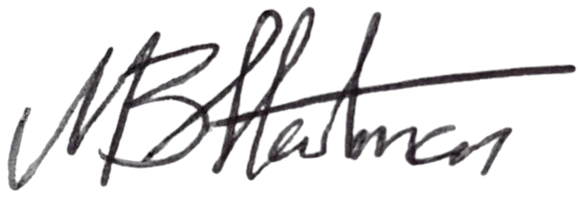
\includegraphics[width=3.5cm]{figures/mich_handtekening.png} &  & \underline{\today} \\
  \textit{Language editor signature}                           &  & \textit{Date}
\end{tabular}

\vspace*{0.5cm}

\textit{Declaration}
\\[2ex]
I, \underline{\eprthecandidatename} understand what plagiarism is and have carefully studied the plagiarism policy of the University. I hereby declare that all the work described in this report is my own, except where explicitly indicated otherwise. Although I may have discussed the design and investigation with my study leader, fellow students or consulted various books, articles or the internet, the design/investigative work is my own. I have mastered the design and I have made all the required calculations in my lab book (and/or they are reflected in this report) to authenticate this. I am not presenting a complete solution of someone else.

Wherever I have used information from other sources, I have given credit by proper and complete referencing of the source material so that it can be clearly discerned what is my own work and what was quoted from other sources. I acknowledge that failure to comply with the instructions regarding referencing will be regarded as plagiarism.  If there is any doubt about the authenticity of my work, I am willing to attend an oral ancillary examination/evaluation about the work.

I certify that the Project Proposal appearing as the Introduction section of the report is a verbatim copy of the approved Project Proposal.

\begin{tabular}{cp{5cm}ll}
  
\includegraphics[width=3.5cm]{figures/anton_handtekening.png} &  & \underline{\today} \\
  \eprthecandidatename                                          &  & Date
\end{tabular}

%% End of File.

